\documentclass[11pt]{article}
\usepackage[margin=1in]{geometry}
\usepackage[T1]{fontenc}
\usepackage{lmodern}
\usepackage{mathtools,amssymb,amsthm,bm}
\usepackage{graphicx}
\usepackage{tikz}
\usetikzlibrary{arrows.meta,positioning}
\usepackage{hyperref}
\hypersetup{hidelinks}
\usepackage{zref-clever}

\graphicspath{{assets/images/}}

\newcommand{\ProjectTitle}{The circulant Hadamard conjecture}
\newcommand{\TeamMembers}{%
  Steven Creech\texorpdfstring{\textsuperscript{1}}{} and
  Tomas Ortega\texorpdfstring{\textsuperscript{2}}{}}
\newcommand{\TeamAffiliations}{%
  \textsuperscript{1}Rutgers University \quad
  \textsuperscript{2}Princeton University}
\newcommand{\CompetitionTrack}{Algebra/Number Theory}
\newcommand{\RepositoryURL}{https://github.com/TomasOrtega/circulant-Hadamard}
\newcommand{\WebsiteURL}{https://tomasortega.net/circulant-Hadamard/}
\newcommand{\SubmissionCommit}{To be set at submission}


\title{\ProjectTitle}
\author{\TeamMembers{} \\ \TeamAffiliations{} \\
  \small Track: \CompetitionTrack{} \\
  \small \url{\RepositoryURL} \\
  \small Commit: \texttt{\SubmissionCommit}}
\date{November 2026}

\begin{document}
\maketitle

\begin{abstract}
  To do: Summarize the question, contribution, and status of the results.
\end{abstract}

\section{Problem and motivation}
We study the circulant Hadamard conjecture~\cite{mathathon}.

A circulant matrix is determined by its first row
\(\bm{a}\coloneqq(a_0,\ldots,a_{n-1})\), with each later row shifted cyclically
by one position. A matrix \(H\in\mathbb{R}^{n\times n}\) with entries in
\(\{-1,1\}\) is Hadamard when
\begin{equation}
  H H^{\mathsf{T}} = n I_n.
  \label{eq:hadamard}
\end{equation}
The identity in \zcref{eq:hadamard} states that distinct rows are orthogonal.

To do: Explain the motivation and prior work.

\section{Contribution and evidence}
To do: Present the argument and label each claim as proved, computed, cited,
Lean-verified, or conjectural. Describe every key figure in words.

\begin{figure}[ht]
  \centering
  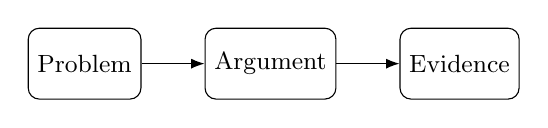
\begin{tikzpicture}[
  node distance=8mm,
  every node/.style={draw, rounded corners, minimum height=9mm, font=\small},
  >={Latex}
]
  \node (problem) {Problem};
  \node[right=of problem] (argument) {Argument};
  \node[right=of argument] (evidence) {Evidence};
  \draw[->] (problem) -- (argument);
  \draw[->] (argument) -- (evidence);
\end{tikzpicture}

  \caption{Template diagram: start with the problem, develop an argument,
    and provide evidence for the resulting claims.}
\end{figure}

\section{Event work and limitations}
To do: Distinguish work done during the event from prior work. State limitations
and next steps.

\section{AI use and acknowledgements}
To do: Credit sources and help. Name AI tools used, their tasks, and how their
outputs were checked.

\bibliographystyle{plain}
\bibliography{references}

\end{document}
